\documentclass[a4paper]{article}

%% Language and font encodings
\usepackage[english]{babel}
\usepackage[utf8x]{inputenc}
\usepackage[T1]{fontenc}

%% Sets page size and margins
\usepackage[a4paper,top=3cm,bottom=2cm,left=3cm,right=3cm,marginparwidth=1.75cm]{geometry}

%% Useful packages
\usepackage{amsmath}
\usepackage{graphicx}
\usepackage[colorinlistoftodos]{todonotes}
\usepackage[colorlinks=true, allcolors=blue]{hyperref}

\title{Evaluación 2}
\author{Isaac Neri Gómez Sarmiento}

\begin{document}
\maketitle


\section{Introducción}
En esta evaluación se simuló el sistema de Lorenz, el cual consiste en un sistema de ecuaciones diferenciales ordinarias. Este tipo de ecuaciones fue estudiada por el matemático Edward Norton Lorenz, cuyas investigaciones se centraron en la teoría del caos.\

Lorenz utilizó su modelo para poder explicar la convección atmosférica, el cual consiste en tres ecuaciones diferenciales ordinarias:


\[\frac{dx}{dt}=\sigma(y-x)\]
\[\frac{dy}{dt}=x(\rho-z)-y\]
\[\frac{dz}{dt}=xy-\beta z\]

Fisicamente lo que describen son las propiedades de un fluído ideal el cual está uniformemente cálido por debajo y frío por arriba. Las variables x, y, z representan  la proporcionalidad de la razon de cambio de la convección, la variación horizontal de la temperatura y la vertical respectivamente. Los coeficientes $\sigma, \rho  y  \beta$ son parámetros físicos los cuales se asumen positivos.

\section{Resultados y discusión}

Se utilizaron 3 valores diferentes para cada uno de los parámetros $\sigma, \rho y \beta$. Donde el primer caso corresponde a los valores que usó Lorenz los cuales presentan comportamiento caótico, incluyendo valores muy cercanos a ellos.

\subsection{Resultados: Primer caso}

\begin{center}
$\sigma=10$ $\beta=8/3$ y $\rho=28$
\end{center}

El atractor de Lorenz en el espacio tridimensional está dado por la siguiente gráfica:

\begin{figure}[ht!]
\centering
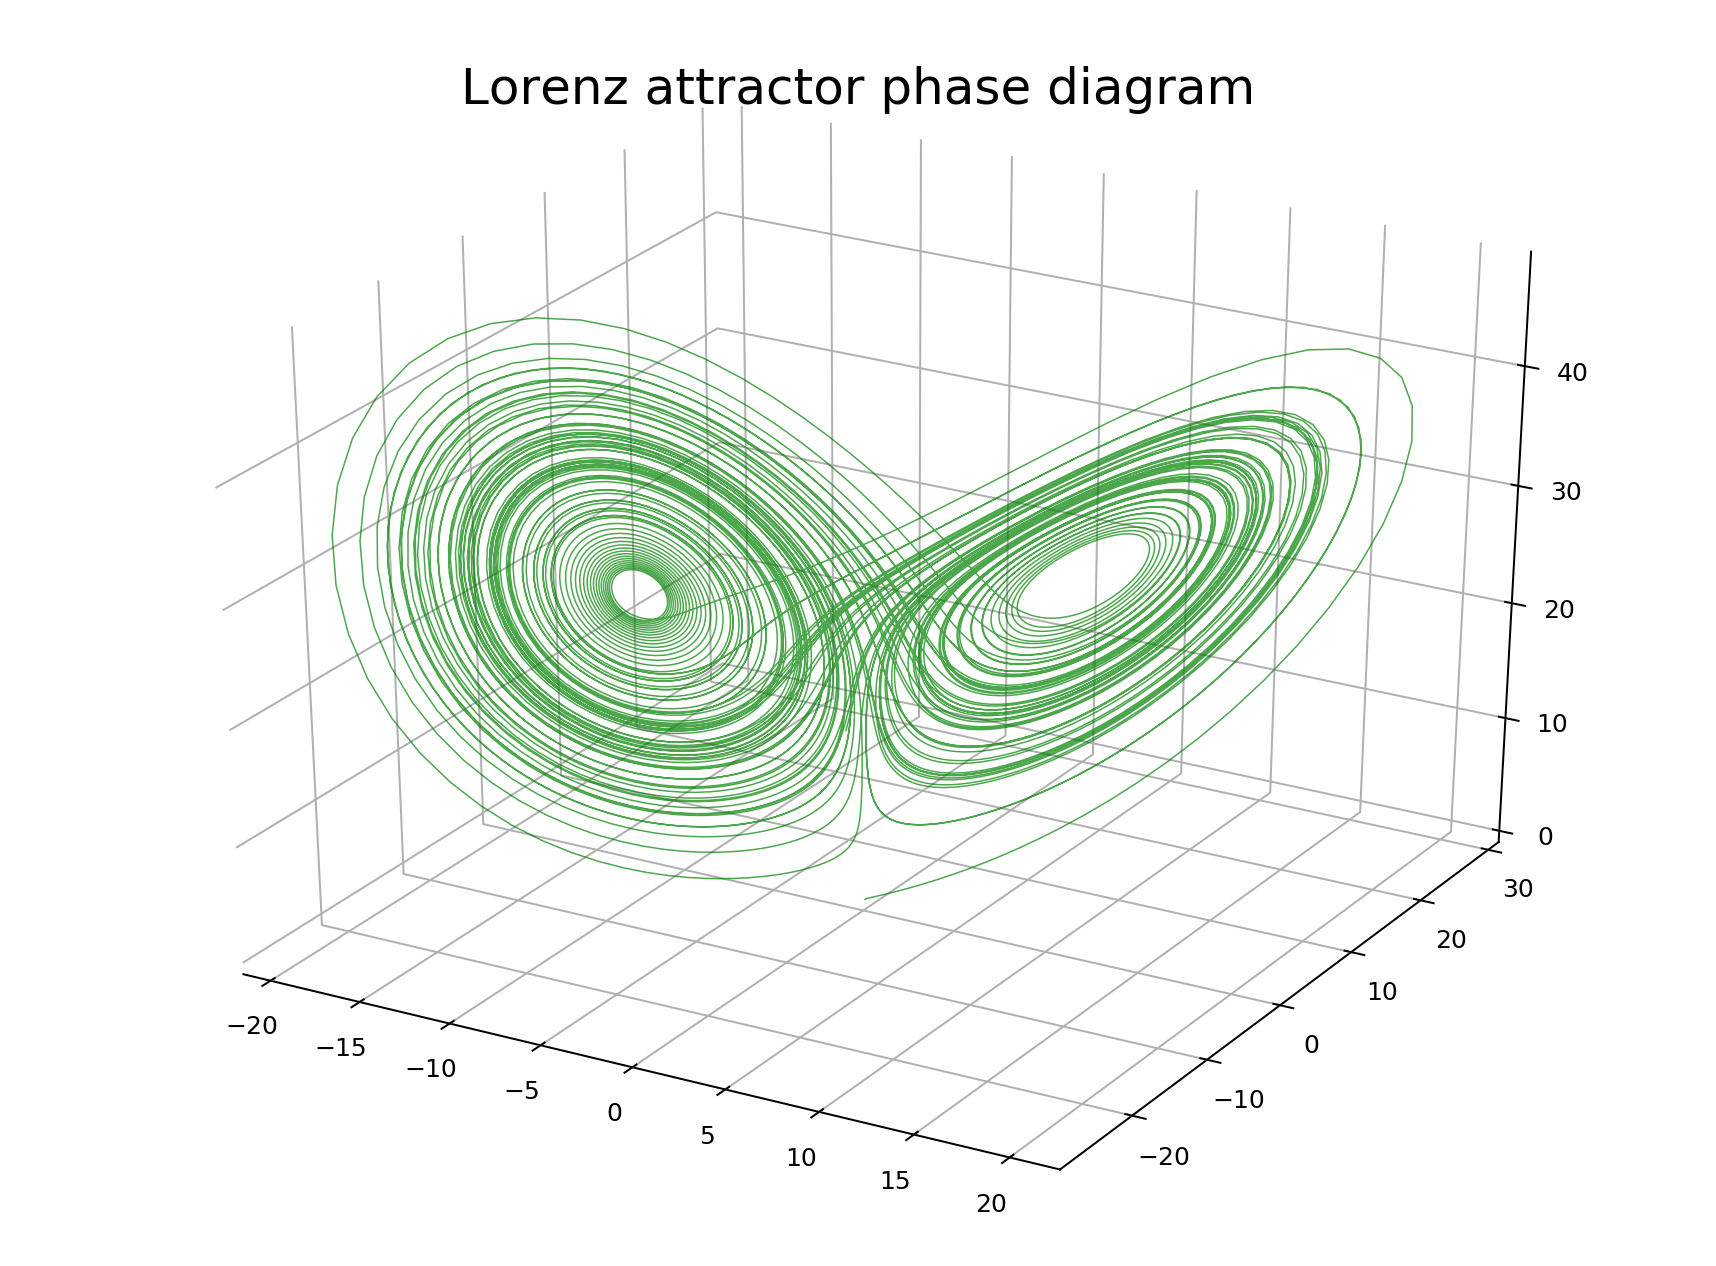
\includegraphics[width=0.5\textwidth]{lorenz-attractor-3d.png}
\end{figure}



\newpage

Se presentan gráficas bidimensionales en cada uno de los planos xy, zy y xz. 

\begin{figure}[ht!]
\centering
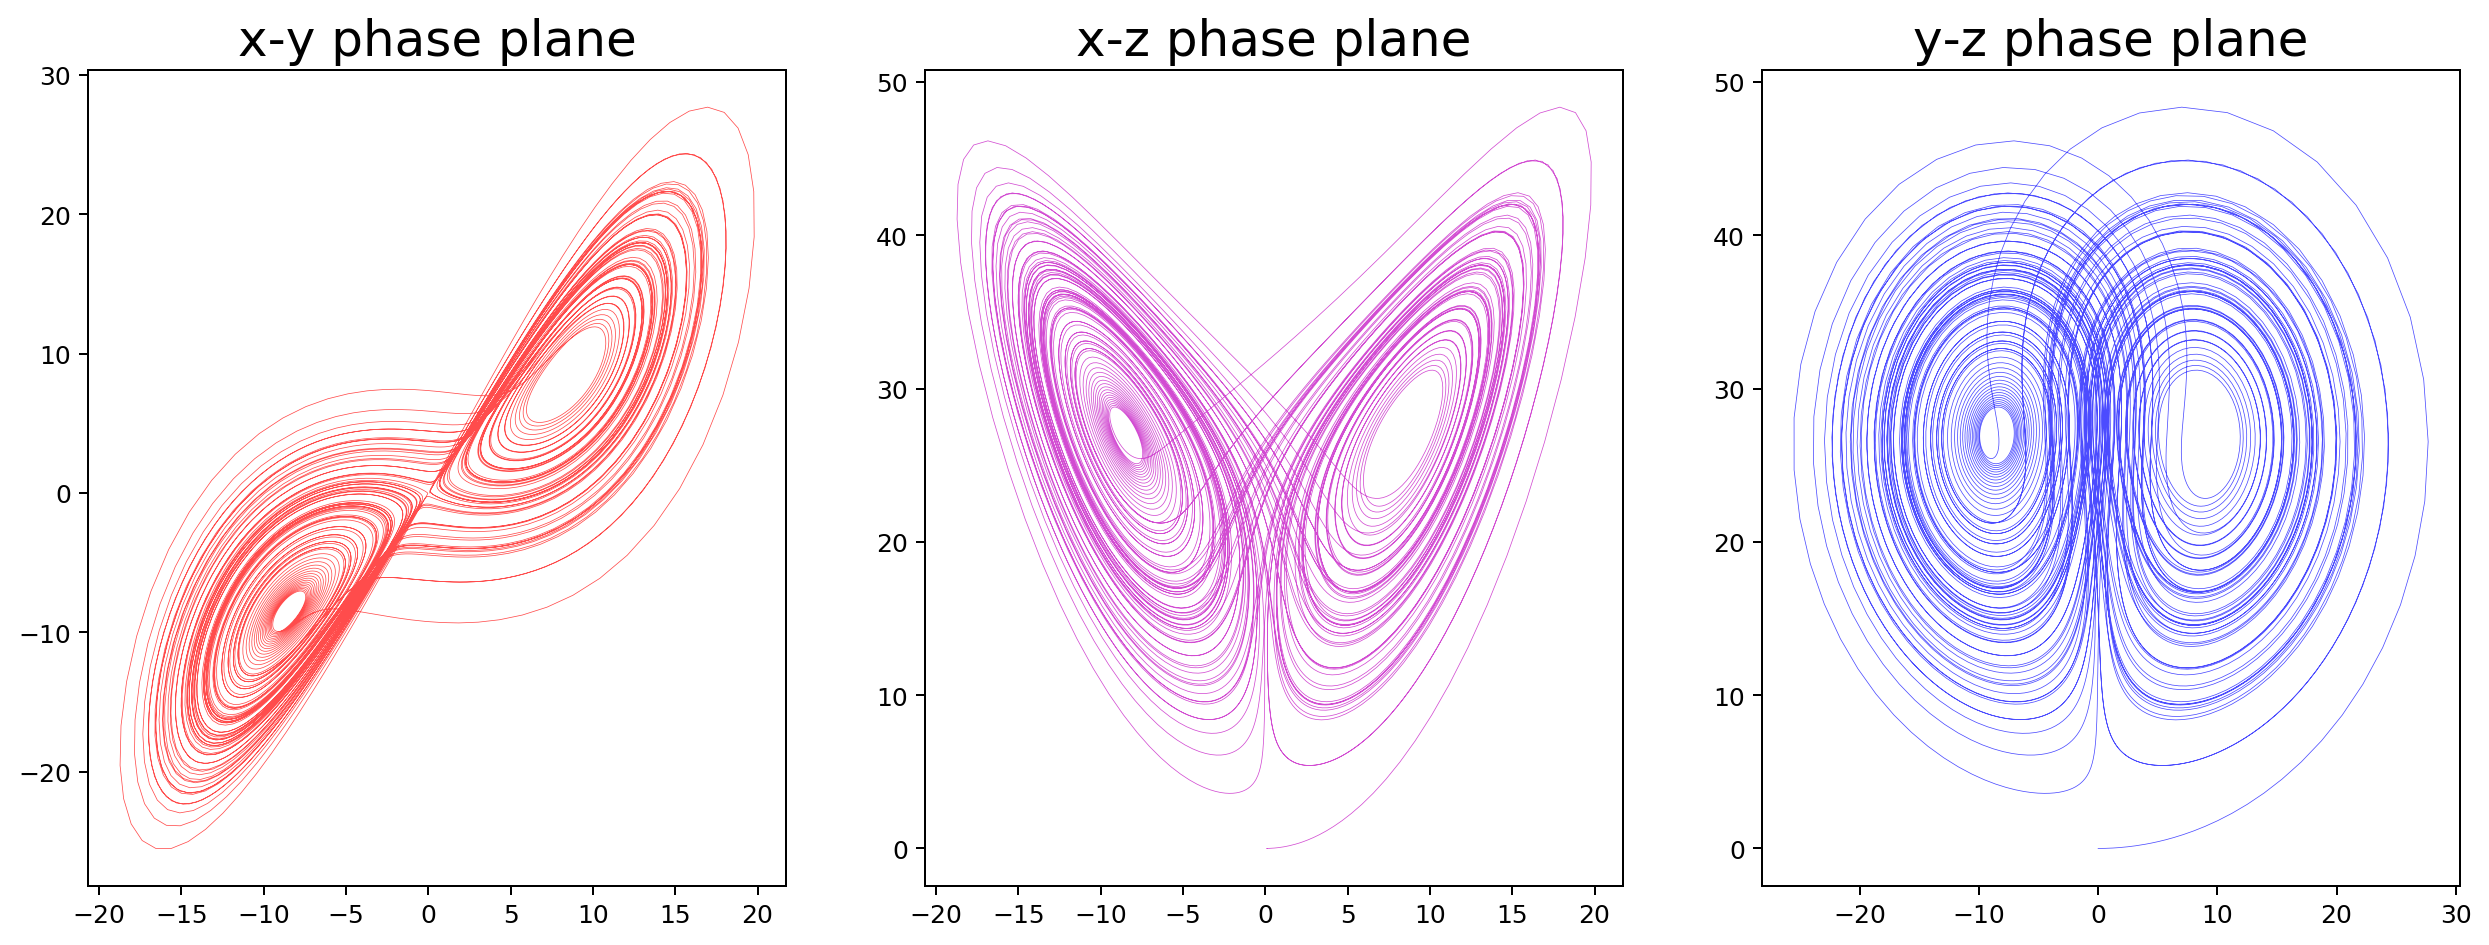
\includegraphics[width=1.0\textwidth]{lorenz-attractor-phase-plane.png}
\end{figure}

Adicionalmente se crearon gráficas bidimensionales de las soluciones x(t), y(t) y z(t) en gráficas separadas y en una sola.

\begin{figure}[ht!]
\centering
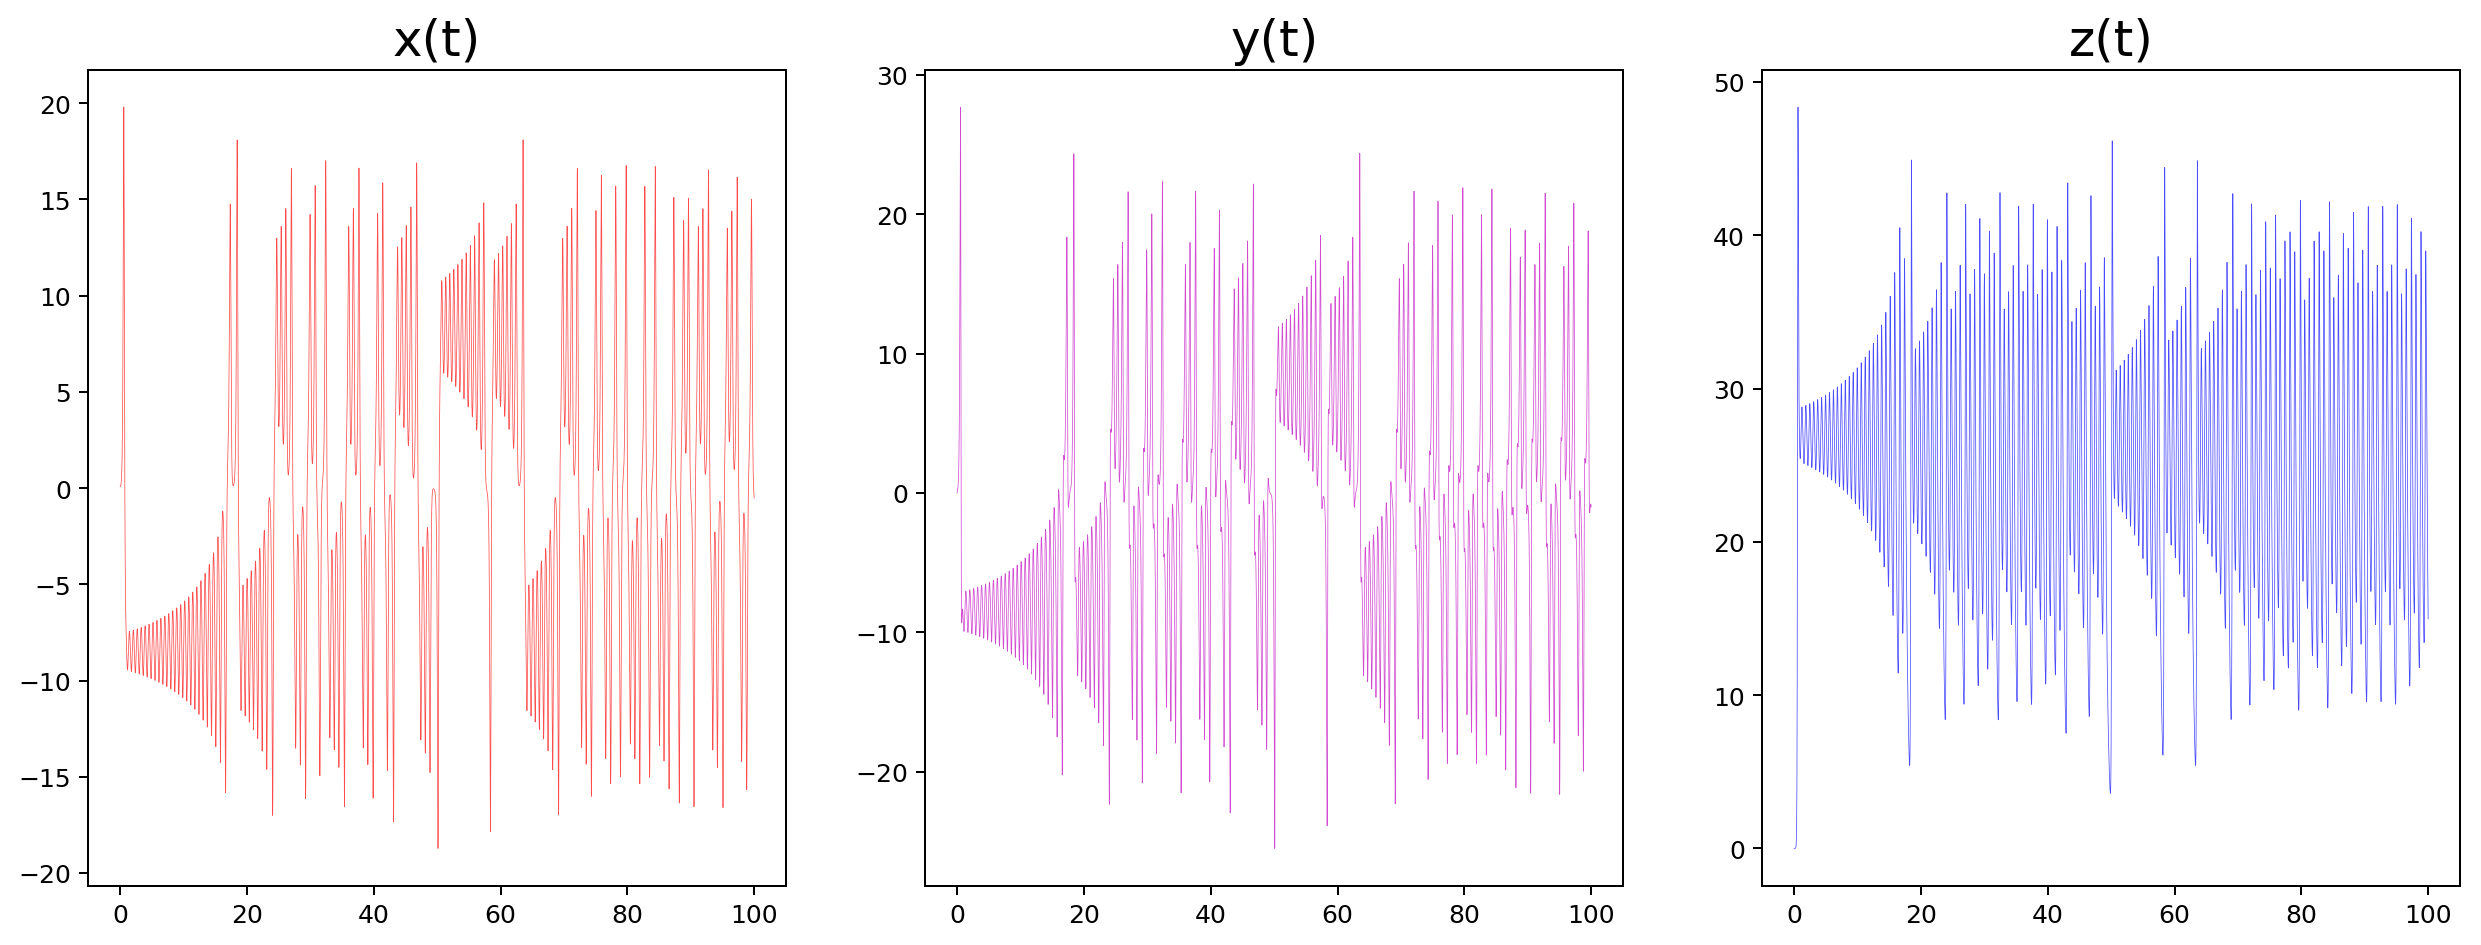
\includegraphics[width=1.0\textwidth]{graficabidimensional.png}
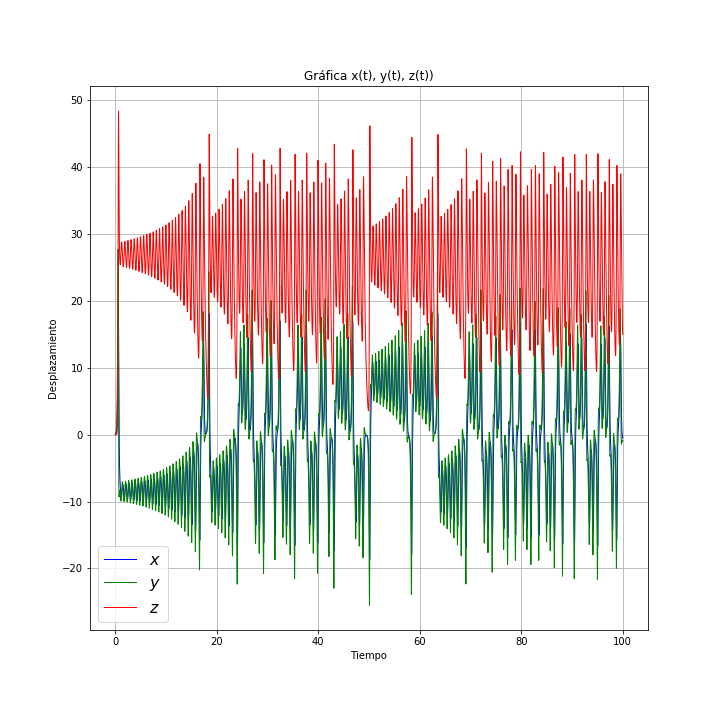
\includegraphics[width=0.5\textwidth]{twodimgraph1.png}
\end{figure}

\newpage

\subsection{Resultados: Segundo caso}

\begin{center}
$\sigma=28$ $\beta=4$ y $\rho=46.92$
\end{center}

El atractor de Lorenz en el espacio tridimensional está dado por la siguiente gráfica:

\begin{figure}[ht!]
\centering
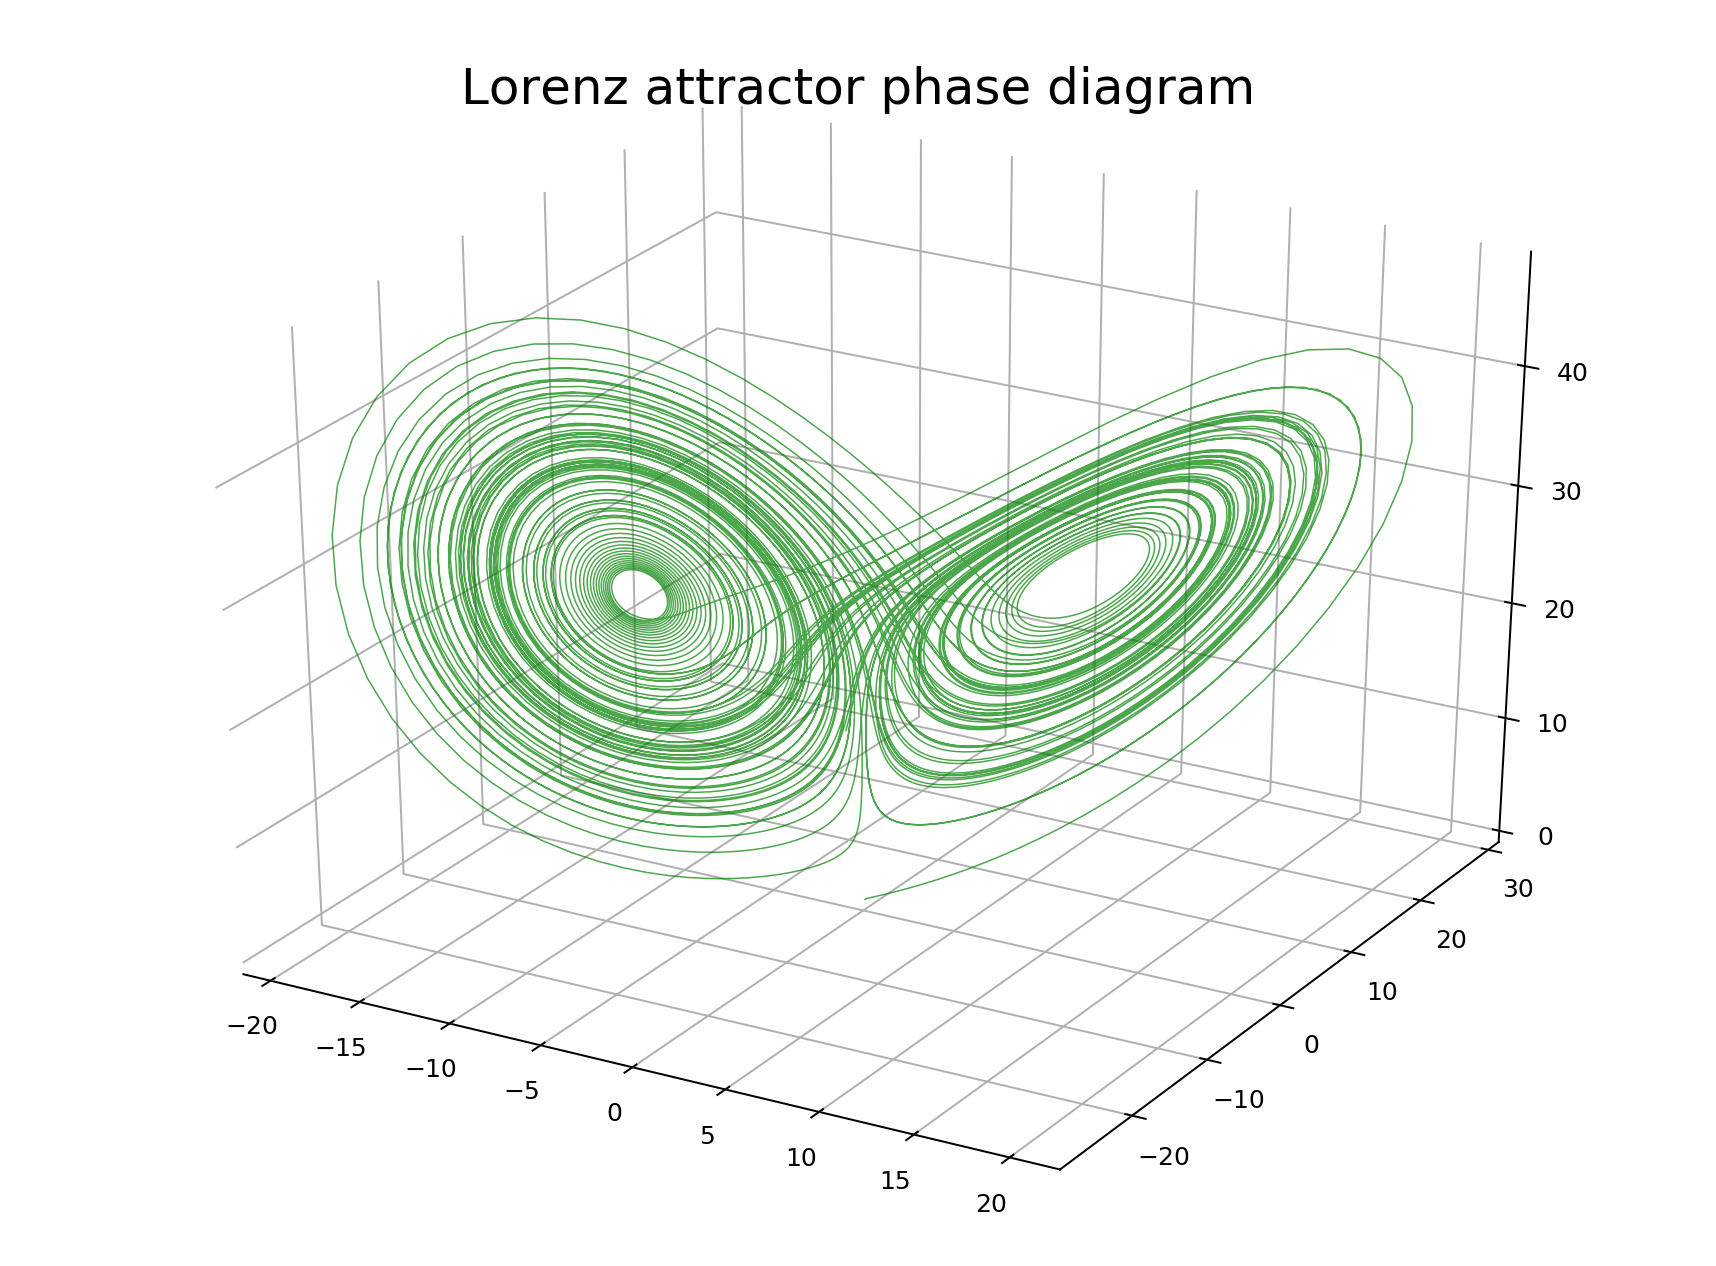
\includegraphics[width=0.5\textwidth]{lorenz-attractor-3d.png}
\end{figure}

Se presentan gráficas bidimensionales en cada uno de los planos xy, zy y xz. 

\begin{figure}[ht!]
\centering
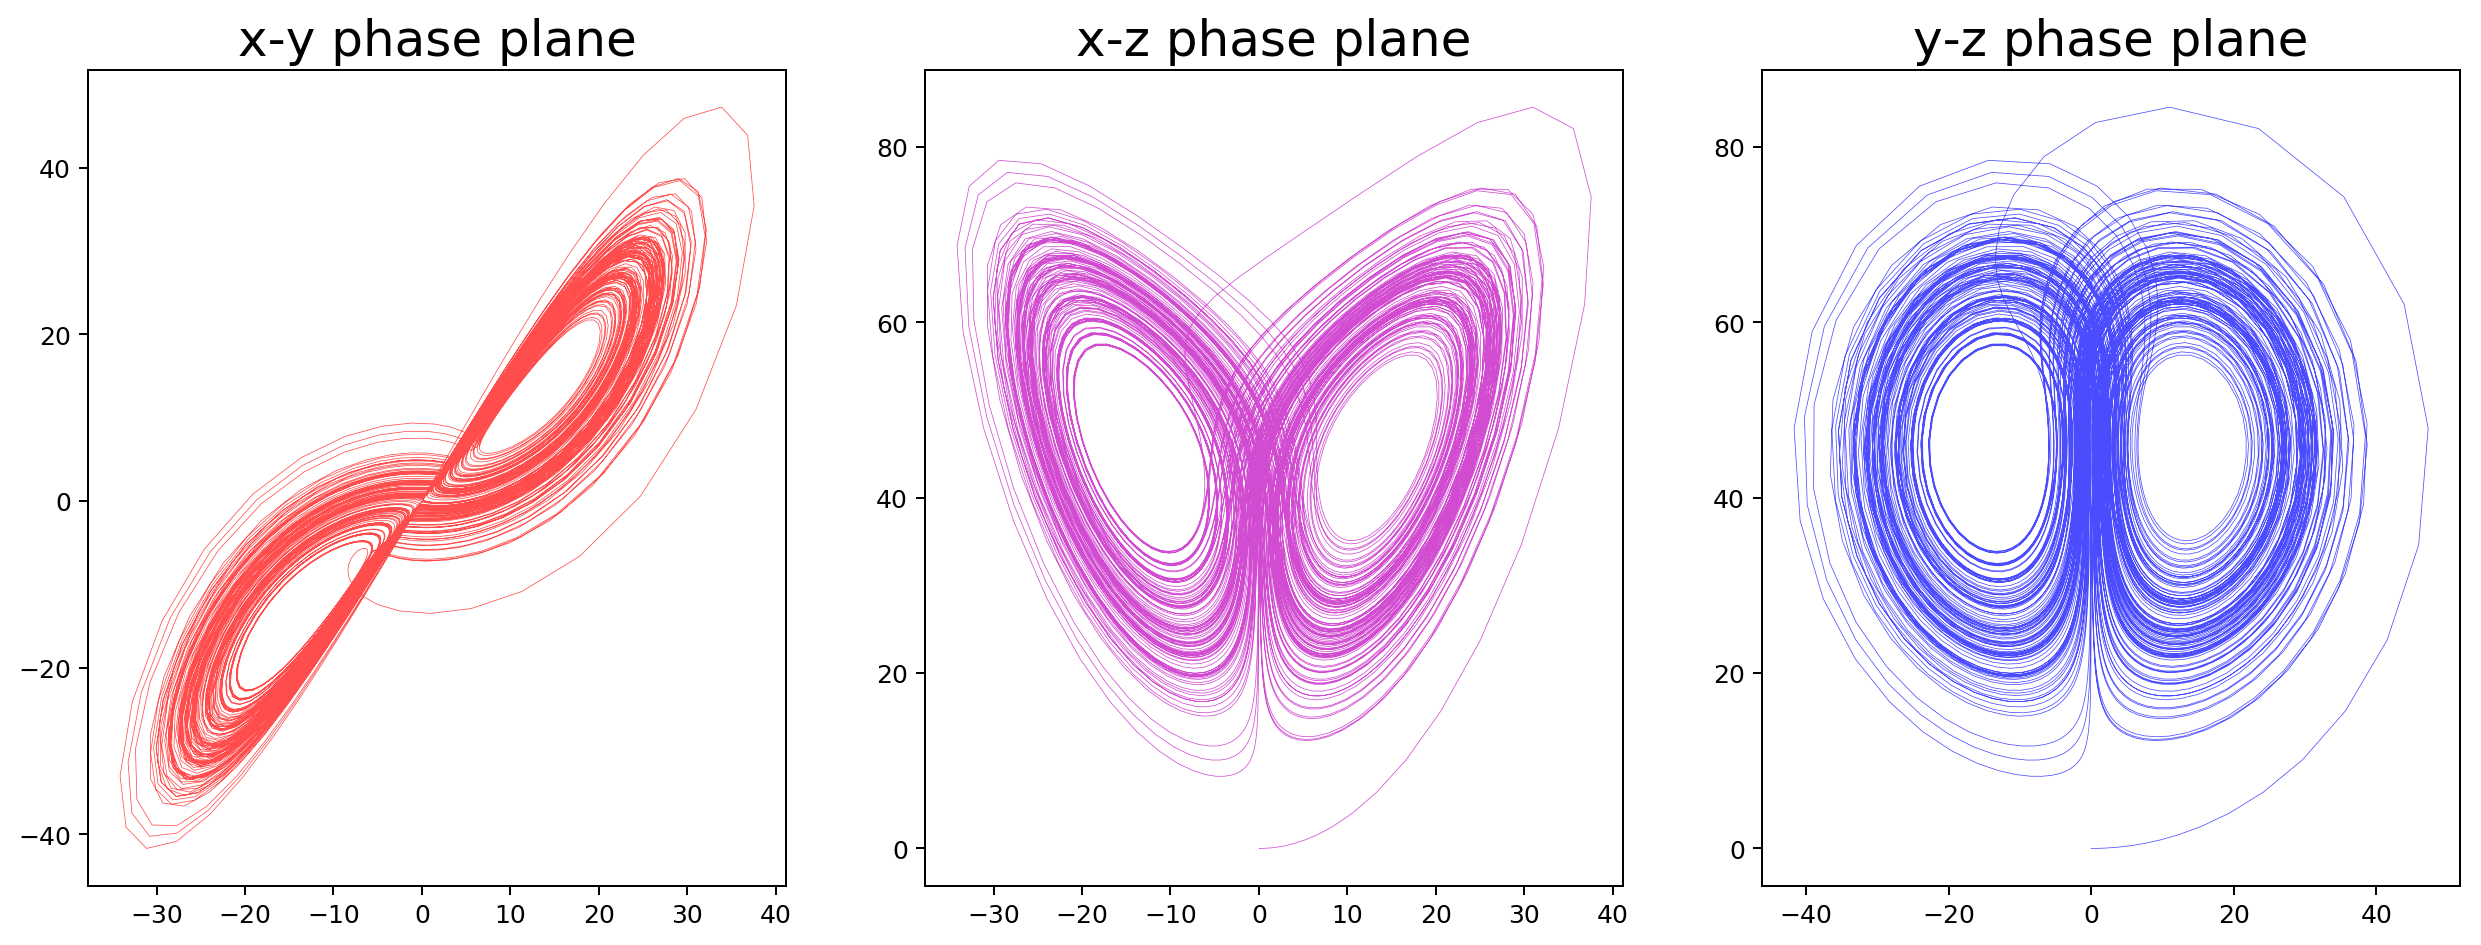
\includegraphics[width=1.0\textwidth]{lorenz-attractor-phase-plane2.png}
\end{figure}

Adicionalmente se crearon gráficas bidimensionales de las soluciones x(t), y(t) y z(t) en gráficas separadas y en una sola.

\begin{figure}[ht!]
\centering
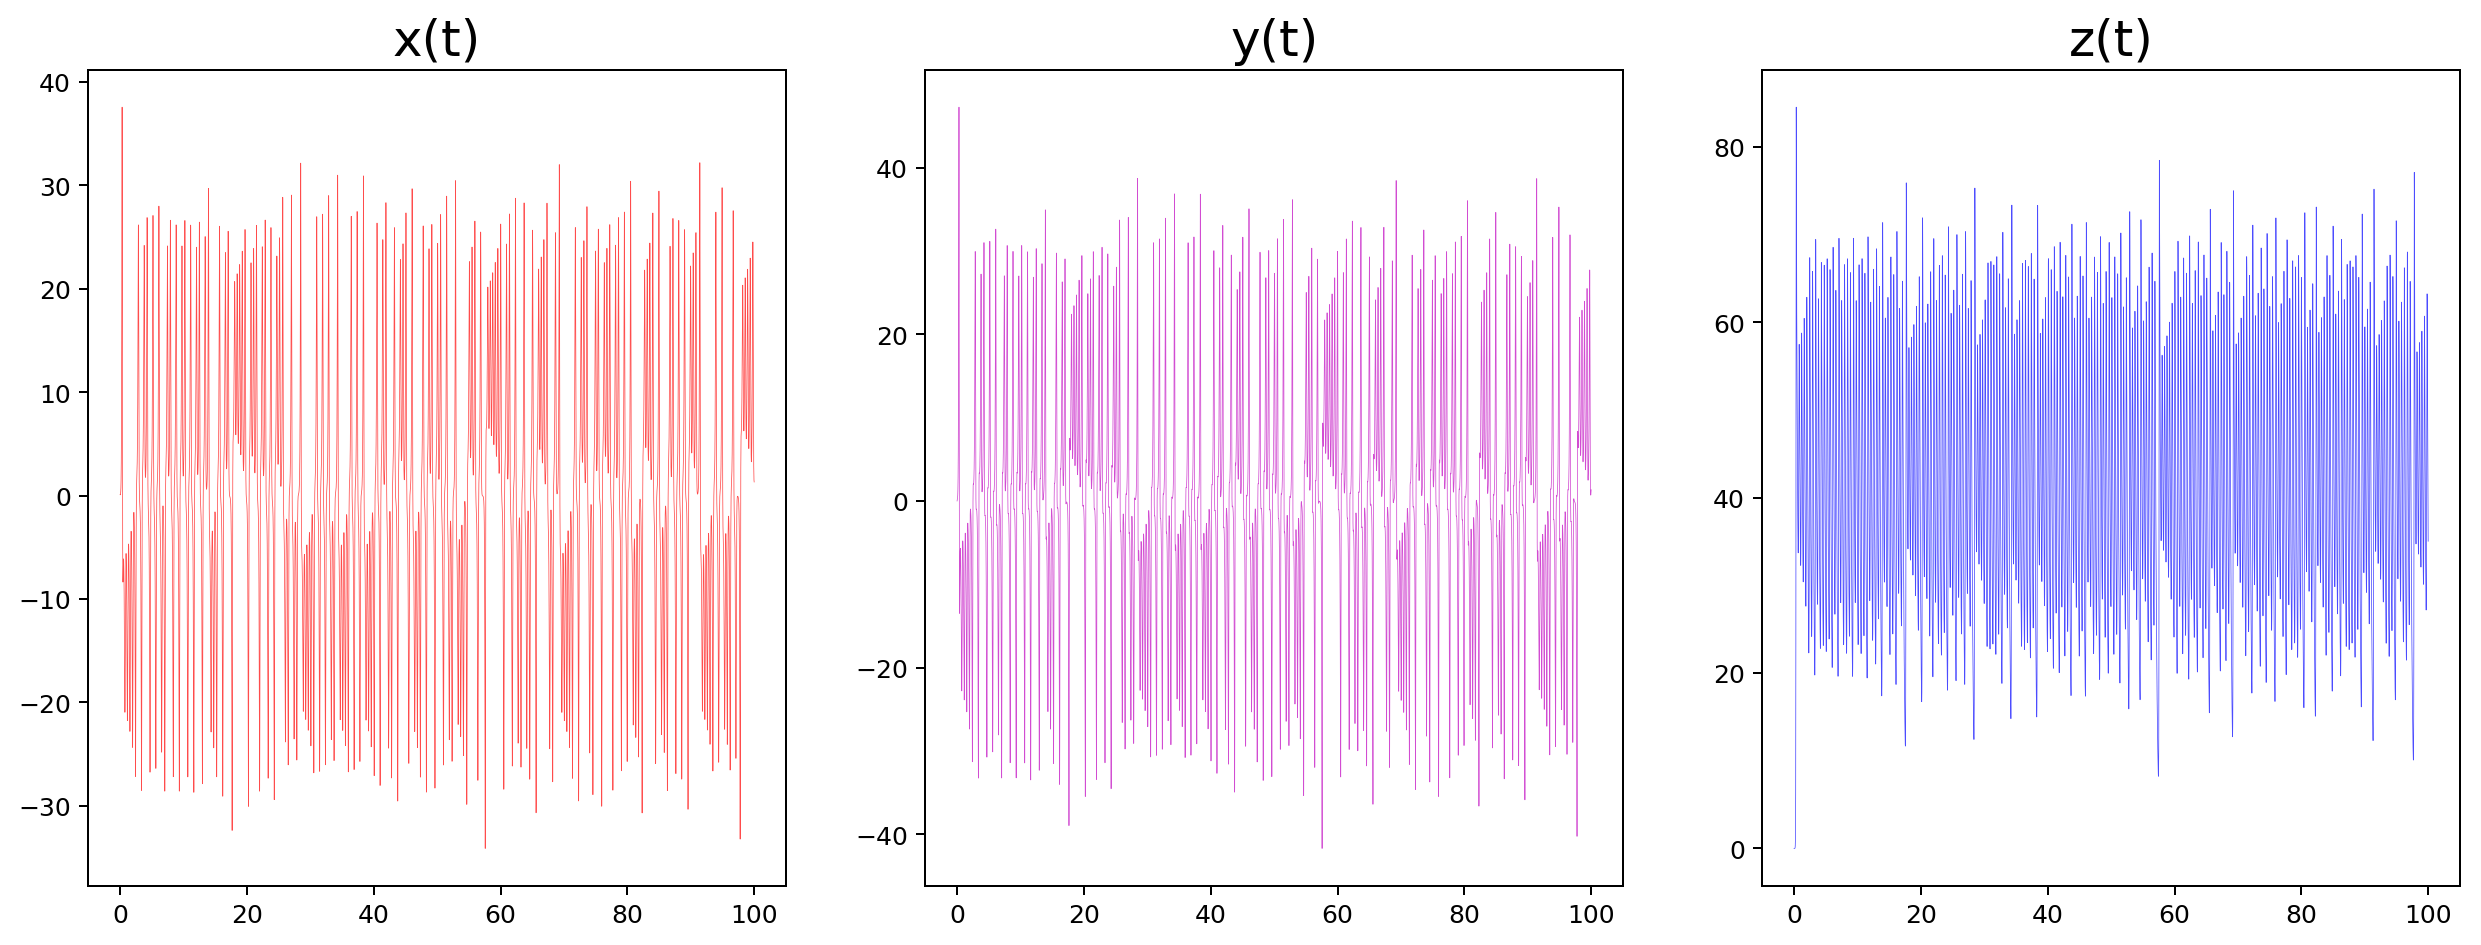
\includegraphics[width=0.7\textwidth]{graficabidimensional2.png}
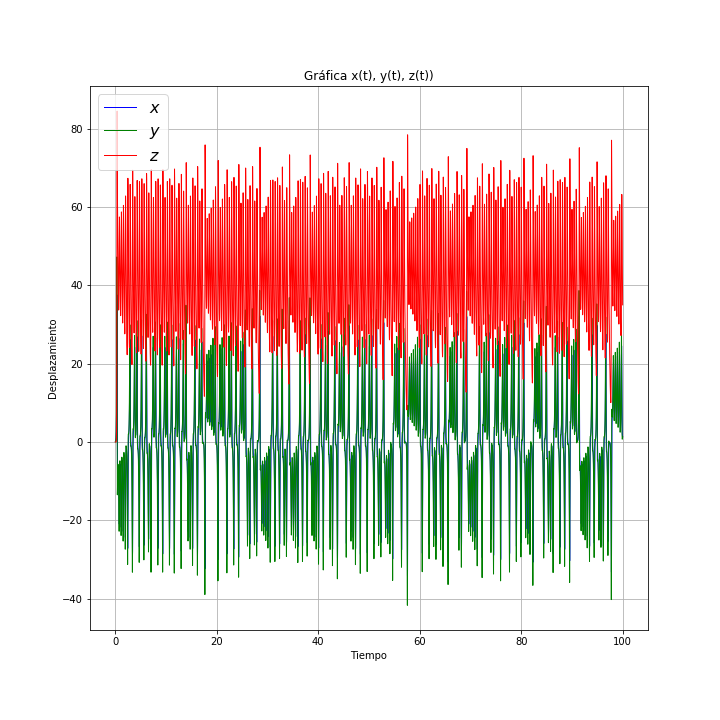
\includegraphics[width=0.4\textwidth]{twodimgraph2.png}
\end{figure}


\newpage

\subsection{Resultados: Tercer caso}

\begin{center}
$\sigma=10$ $\beta=8/3$ y $\rho=99.96$
\end{center}

El atractor de Lorenz en el espacio tridimensional está dado por la siguiente gráfica:

\begin{figure}[ht!]
\centering
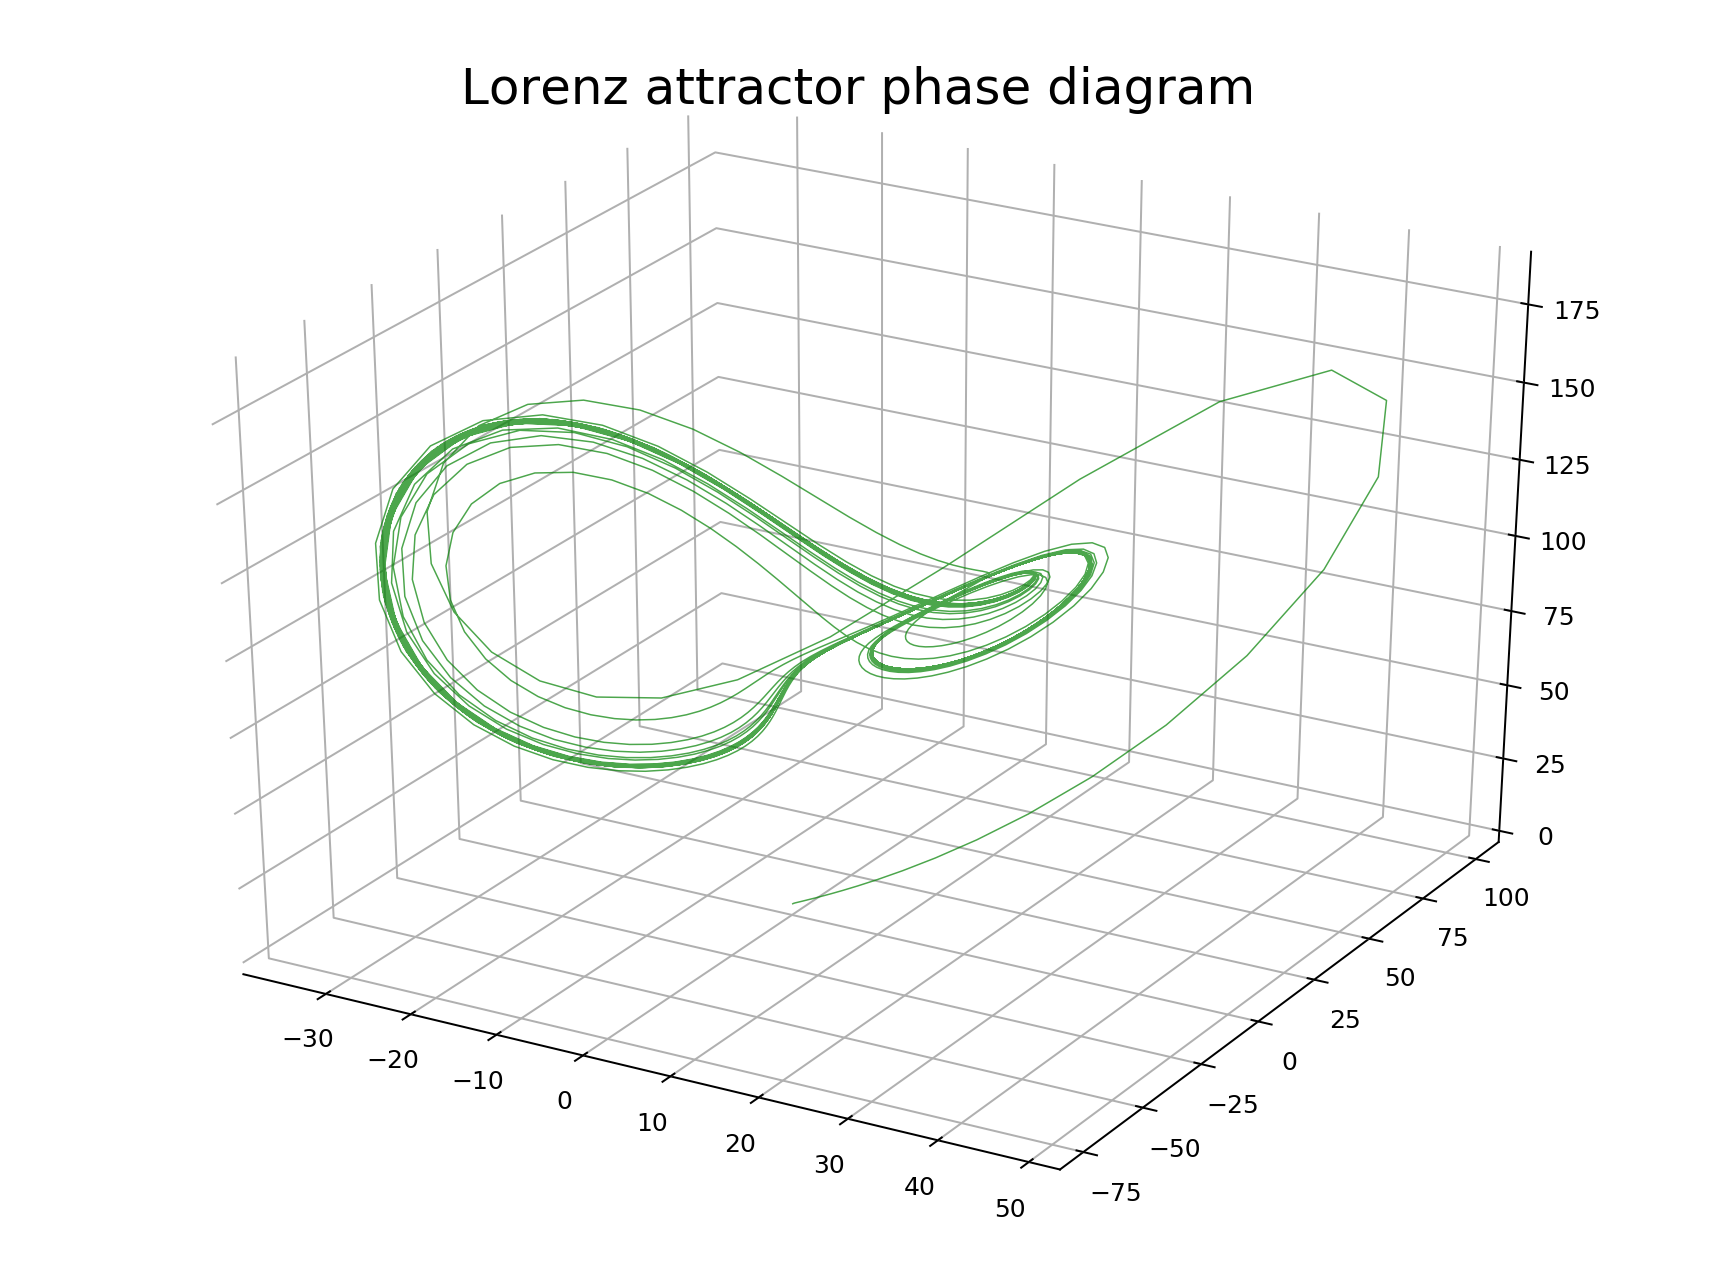
\includegraphics[width=0.5\textwidth]{lorenz-attractor-3d3.png}
\end{figure}

\newpage

Se presentan gráficas bidimensionales en cada uno de los planos xy, zy y xz. 

\begin{figure}[ht!]
\centering
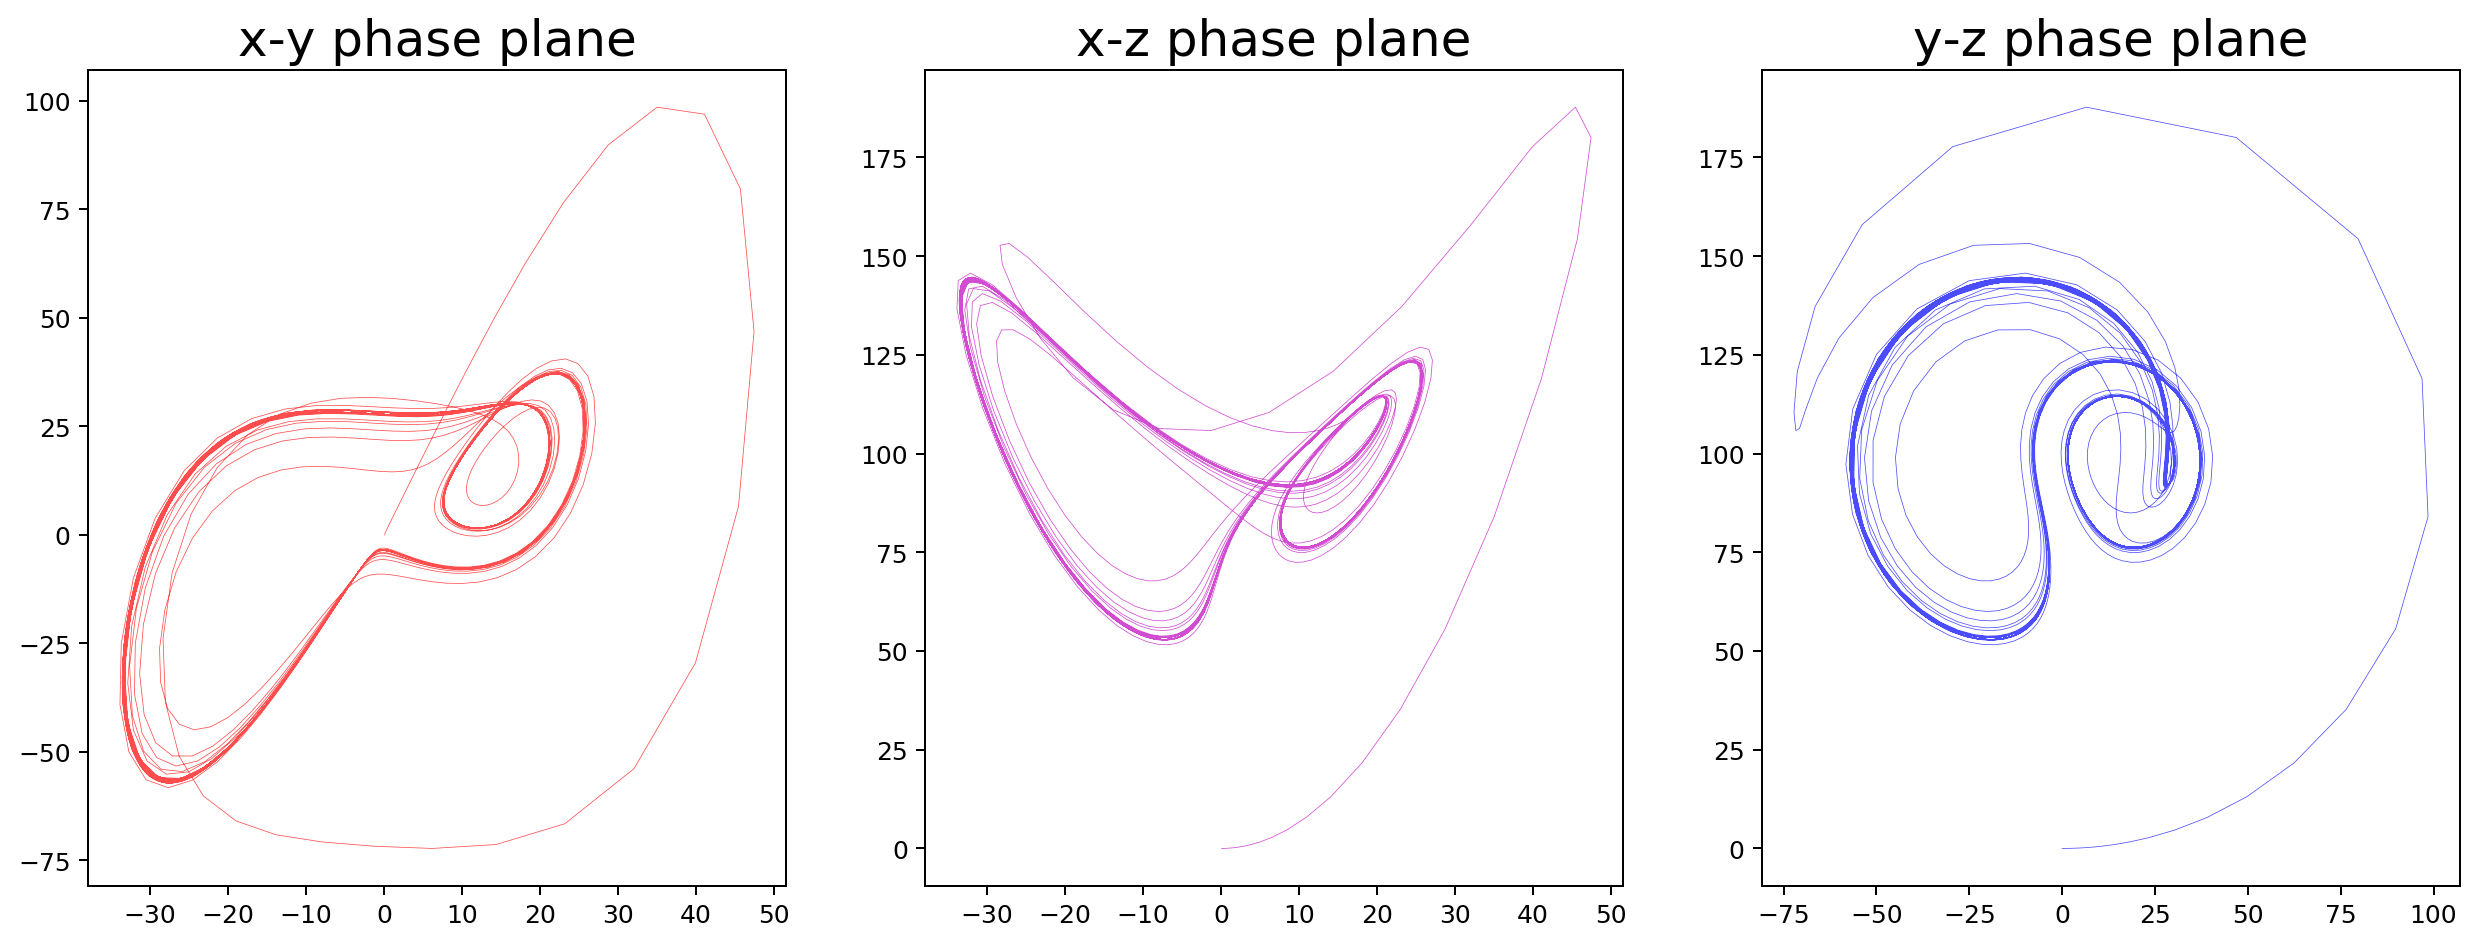
\includegraphics[width=1.0\textwidth]{lorenz-attractor-phase-plane3.png}
\end{figure}

Adicionalmente se crearon gráficas bidimensionales de las soluciones x(t), y(t) y z(t) en gráficas separadas y en una sola.

\begin{figure}[ht!]
\centering
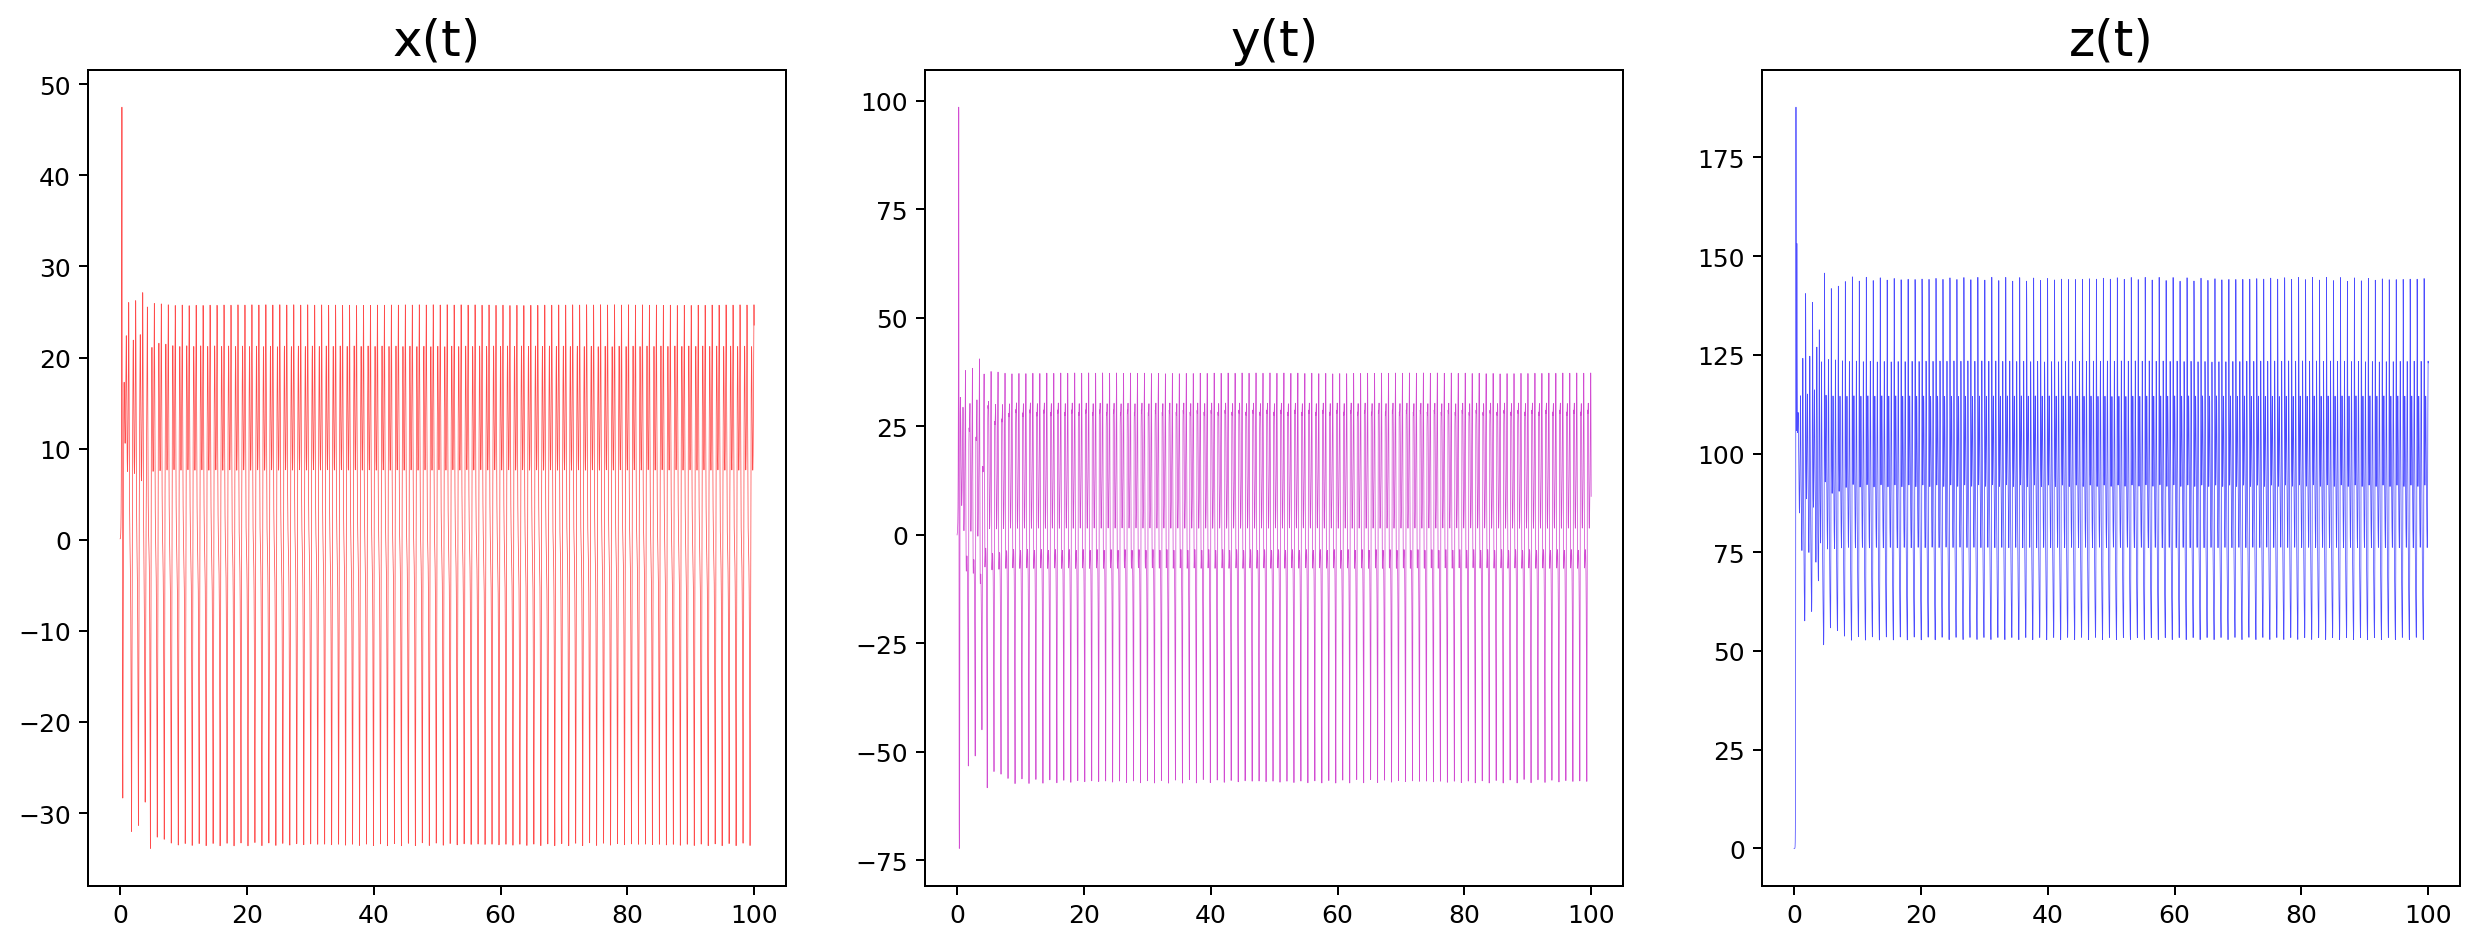
\includegraphics[width=1.0\textwidth]{graficabidimensional3.png}
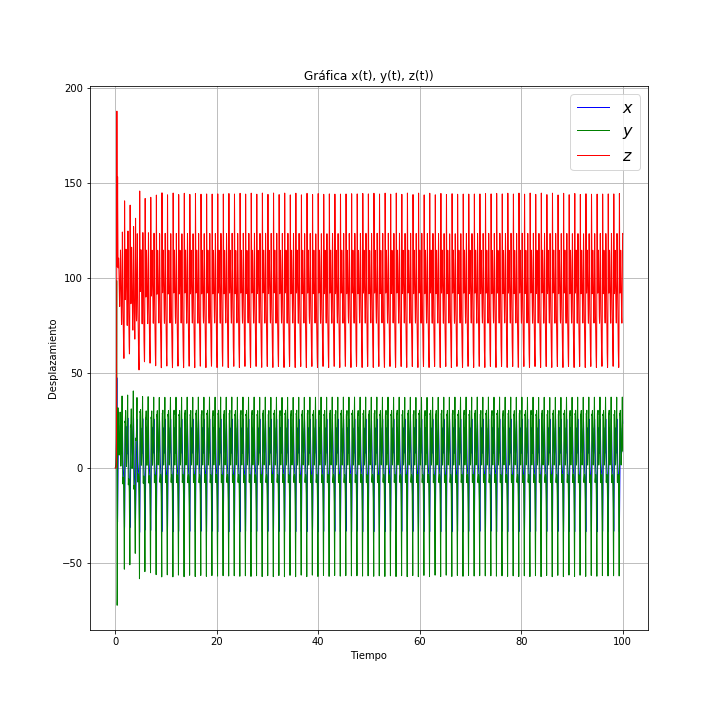
\includegraphics[width=0.7\textwidth]{twodimgraph3.png}
\end{figure}


\subsection{Discusión}

En el segundo caso se aprecia que el atractor incrementa su tamaño, lo cual se debe al aumento del valor de los parámetros en comparación al primer caso. 
En el primer caso, el orificio de la izquierda es más pequeña que el de la derecha. Si lo contrastamos con el atractor del segundo caso, podremos apreciar que el orificio de la derecha es un poco más grande que el de la izquierda. 

A pesar de mantener el caso tres los valores de $\sigma$ y $\beta$ iguales que los del caso uno, la forma del atractor del caso tres cambia drásticamente, además de tener las curvas más cercanas que en el caso uno. 

En cuanto a las gráficas bidimensionales de soluciones x(t), y(t), z(t), llama la atención que en la gráfica del caso tres las oscilaciones no llegan a valores cercanos a 50, además que la variación de las variables x y y están muy cercanas entre sí, mientras que para la variable z, necesita más tiempo para poder llegar a intersectar a las gráficas de las variables x y y.


\section{Conclusión}

El atractor de Lorenz no solo tiene un aspecto vistoso tal como el de una mariposa, sino que resulta ser una herramienta en la física como la predicción del clima. Tal y como se pudo notar,  al cambiar un poco los valores iniciales, parece desviarse los resultados muy rapido. No obstante, según el propio Lorenz dijo que su sistema es determinista, lo cual significa que si sabes exactamente los valores de inicio, entonces puedes predecir futuros valores. En sí, las curvas que se generan representan las trayectorias tomadas por un estado físico particular representado por un punto.




\section{Bibliografía}

Lorenz system. Wikipedia. Recuperado el 26/04/2018 de: \url{https://en.wikipedia.org/wiki/Lorenz_system}

The Lorenz Attractor. Recuperado el 26/04/2018 de: \url{http://homepages.math.uic.edu/~kjerland/Lorenz/lorenz_attractor.html}

\end{document}